\documentclass[12pt]{article}
\usepackage[right=1.25in,left=1.25in,top=1.1in,bottom=1.1in]{geometry}
\usepackage{hyperref}
\hypersetup{colorlinks, citecolor=blue, filecolor=blue, linkcolor=blue, urlcolor=blue}
\usepackage{graphicx}
\usepackage{url}
\usepackage[round]{natbib}
\usepackage{amsmath,amsthm} 
\usepackage{engord}
\usepackage{float}
\usepackage{subfig}
\usepackage{pdflscape}
\usepackage{booktabs}
\usepackage{pgfplots}
\pgfplotsset{compat=1.14}
\pgfplotsset{every axis label/.append style={font=\tiny}}
\usepackage[labelsep=period]{caption}
\usepackage{amssymb}
\usepackage{multirow}
\usepackage{xr}
\usepackage{setspace}
\onehalfspacing
\usepackage{sectsty}
\sectionfont{\large}
\subsectionfont{\normalsize}
\subsubsectionfont{\normalsize}
\newcommand{\specialcell}[2][c]{\begin{tabular}[#1]{@{}l@{}}#2\end{tabular}}

\title{ \vspace*{-2.5cm} \hspace*{-0.5cm} Would Origin and Type of Undergraduate Universities Affect Ph.D. Ranking? Evidence From 2021-2022 Job Market\footnote{
}}

\author{Yubo Wei \\ Econ 196 Thesis\\
Professor Shelly Lundberg \\
Advisor Dick Startz}


\date{ \vspace*{0.5cm} March, 2022\\
} 
\title{ \vspace*{-2.5cm} \hspace*{-0.5cm}Would Origin and Type of Undergraduate Universities Affect Ph.D. Ranking?\\ Evidence From 2021-2022 Job Market\footnote{
I would like to thank Professor Shelly Lundberg and Dick Startz for their incessant support for this research during this 6 month period. I appreciate their advice and guidance on intellectual stimulation. They help keep the process on the right track. This study cannot be done without their generous help.
}}

%%%%%%%%%%%%%%%%%%%%%%%%%%%%%%%%%%%%%%%%%%%%%%%%%%%%%%%%%%%%%
\begin{document}

\bgroup
\let\footnoterule\relax

\begin{singlespace}
\maketitle


\begin{abstract}
    \noindent The proportion of international Ph.D. candidates has been increasing in recent years, and the growing importance of international candidates requires researchers to pay more attention to the differences between them and American candidates. Using information collected from CVs on the 2021-2022 economics Ph.D. job market, we find that international candidates are more likely to have a previous graduate degree before a Ph.D., and less likely to have full time RA experiences and a background in math. The results of this study suggest that several variables have positive effects on Ph.D program rankings: graduating from a highly ranked undergraduate institution, having full time RA experiences, and coming from Western Europe, Eastern Europe, or Latin America, while candidates attending an unranked undergraduate institution and an liberal arts college are less likely to graduate from highly ranked Ph.D. programs.
    
\end{abstract}
\end{singlespace}
\thispagestyle{empty}

\clearpage
\egroup
\setcounter{page}{1}


\section{Introduction\label{sec:introduction}}

\noindent Every year economics departments in the U.S. award hundreds of Ph.D. degrees to students from around the world. While the total number of Ph.D.s awarded has remained between 850 and 1150 per year since 1970, the number of U.S. citizens earning a Ph.D. in economics from an American university has declined steadily for three decades, falling from a peak of 852 in 1973 to a low of 396 in 2003 \citep{stock2007}. Diminished perceptions and difficulties securing visas for study in the U.S. in the recent years have not influenced the demographic transition of economics Ph.D.s. From 2017 to 2022, the proportion of international candidates in the top 50 Ph.D. programs rose from 54.2 percent \citep{pathtoeconphd} to 62 percent. Therefore, the increasing importance of international candidates requires researchers to pay more attention to some of the characteristics they differ from those of American candidates.

This paper empirically investigates whether several characteristics unique to international candidates influence their Ph.D. program rankings, using the data from individual CVs posted by top 50 Ph.D. programs in the 2021-2022 job market. The first characteristic is the type of undergraduate school the candidate is enrolled in. We rank all universities based on whether they are ranked in the 2016 QS world ranking, dividing them in four categories: ranked, unranked, undergraduate economics school, and liberal arts colleges. Undergraduate schools of economics are mainly from Italy, the United Kingdom, and Russia, while the liberal arts colleges are limited to American students. The 2016 QS world ranking surveys about 700 undergraduate schools, the ones that aren't included will be classified as unranked. We find that if an undergraduate institution moves up 100 places in the rankings, the candidate's Ph.D. program will move up about 1.9 places. Attending an unranked undergraduate school lowers the Ph.D. program's ranking by about 12 places,  while attending an liberal arts college and an undergraduate economics school do not have significant effects on the Ph.D. program rankings. The second is the region of origin. The foreign sources of U.S. Ph.D. candidates are divided into six major regions, Western Europe, Eastern Europe (CIS), Latin America, South Asia, and East Asia. We find that undergraduate institutions from Western Europe, Eastern Europe, and Latin America increase the ranking of doctoral programs by 7.6, 8.2, and 7.3 places, respectively, while other regions show no significant impact on the rankings.

As part of the data analysis, the effect of pre-admission characteristics has also been studied. We examine several parameters directly derived from the CVs, namely candidates' academic backgrounds and post-baccalaureate experiences and address the difference between U.S. candidates and international candidates. We find that compared with U.S. candidates, international candidates are less likely to have a math background, less likely to hold full-time research experiences, and more likely to complete a master's degree before earning the Ph.D. degree. We also explore the effect of pre-admission characteristics on Ph.D. program rankings. We find that, surprisingly, if we just looked at the data, 86.9 percent of candidates at 1-5 ranking tier had an economics background, while the proportion of graduates from lower-ranked programs with an economics background was above 90 percent, or even 100 percent. As a results, candidates with an economics background ranked their Ph.D. programs on average about 4.8 places lower than those without an economics background. Having a math background increased the ranking by about 1.7 places, but the result was not significant.

The remainder of the paper is organized as follows. Section 2 we revisit previous related research. Section 3 consists our analysis of the data, including descriptive statistics for updated database and analysis of new variables. Section 4 discusses the our empirical strategy and the results and section 4 concludes.

\section{Literature Review \label{sec:literature review}}
The search for talent is a topic of particular interest to economists. While related topics are discussed by scholars every once in a  while, different conclusions are usually drawn. For instance, using data from 48 institutions’ 1990 and 1991 applicant pools, \citet{Attiyeh1997TestingFB} regress acceptance on academic and demographic characteristics, and find that GRE, GPA, a related undergraduate major, and holding a master’s degree have a statistically significant impact on the probability of acceptance. They also find that conditional on other characteristics, being a female or non-Asian minority significantly increases the probability of acceptance into an economics Ph.D. program. However, recent studies by \citet{stock2007}, \citet{pathtoeconphd} and \citet{jones2020}, find that holding a master’s degree is relatively unimportant for application for students graduated from American Institutions. Schlauch and Startz estimate that only 14\% of Ph.D. candidates from top 50 programs have a master’s degree before Ph.D. admission, and those at highly ranked Ph.D. programs are even less likely to, although the reverse is true for international candidates and also being a male brings a higher chance to graduate from top Ph.D. programs.

Researchers also use pre-acceptance data from admitted students to predict doctoral degree completion and research productivity given that post-acceptance data such as course grades are mostly confidential. Some studies found that the quality of undergraduate institution has effects on graduate education and time for doctoral completion \citep{Tuckman1990}. Math GRE scores are proved to be highly significant in the Ph.D. program admission \citep{Attiyeh1997TestingFB, wu2000} but failed to predict Ph.D. graduation rate or time to finish based on 24 years of economics Ph.D. students at Cornell University \citep{Ehrenberg1995}. However, \citet{wu2007} found that GRE math scores, the undergraduate institution attended, and the quality of reference writers predict doctoral completion and publishing success, by using information from all 344 applications to Princeton University’s economics Ph.D. program in 1989 and tracking their activities 15 years later, then they argue that censored data may explain the differences in results.

Two types of information contained in the Ph.D. applications largely have been ignored in studies of graduate student success: the personal statement and the strength of recommendation letters. In one of the exceptions, \citet{Dutkowsky2007} code the personal statements according to whether the applicant demonstrated an interest in doing economics research, mentioned a specific topic of research interest, and listed one or more department members whose work interested them.  They found research motivation in the personal statement and math preparation to be important explanatory variables for completing the dissertation. In addition, they also discover that high GRE scores, having a Masters degree, and a prior focus on economics appear as significant determinants for passing the comprehensive exams. Letters of recommendation, by contrast, were often deliberately excluded from the analysis of graduate success. One of the reasons is that letters could not accurately predict future success due to leniency \citep{letters1980} and lack of letter writer and of letter reader reliability.

Regarding international students, both \citet{Attiyeh1997TestingFB, wu2000} found that admission committees prefer U.S. citizens over most international applicants, and \citet{Tuckman1990} used data from National Science Foundation's Survey of Earned Doctorates records and found that students from foreign undergraduate institutions took longer to complete Ph.D. degree, and in more recent studies, \citet{pathtoeconphd,stock2014} found no evidence that international students are more or less likely than Americans to graduate from a top 15 Ph.D. program. Despite the implications of such an option being used in the prediction of the Ph.D. admission and time to finish degree, to the best of my knowledge, no paper has divided international candidates into regions based on their undergraduate institutions to examine whether there is a relationship between Ph.D. graduation and regions. Although, consistently, GRE math score, math preparation, undergraduate institution quality, being international are proved to be good predictors of successful outcomes over the last 30 years, factors related to the academic environment may have changed time to time.

This paper makes three contributions to the related topics. First, by collecting data from CVs of the 2021-2022 job market of top 50 economics Ph.D. programs, we create an updated database from \citet{pathtoeconphd} and document the types of undergraduate colleges and universities attended by those who earned a Ph.D. from an American university in 2021. Inferences and recommendations made to students based on a more current and representative sample of graduate school programs can provide additional insights into the admissions process. Second, we associate international candidates from different rankings of Ph.D. programs with the regions of their undergraduate institutions. The origin of the candidates along with their pre-doctoral experiences are also presented by region. To my best knowledge, no paper has done similar division before. One exception comes from \citet{stock2007}, but they only subdivide the foreign institutions into two groups: (a) Britain, Canada, Ireland, Australia, and New Zealand, where English is the dominant language; and (b) all other countries, while we will divide by regions. Finally, we use dummy variables to code undergraduate economics schools that do not have a ranking. Previous studies have largely overlooked the growing influence of these institutions and lumped them together with non-ranking undergraduate colleges.

\section{Data \label{sec:data}}
\subsection{Description}

The data for this paper come primarily from two types of sources. First we collect a census of economics Ph.D. candidates posting curriculum vitae for the 2021-2022 job market from top 50 economics Ph.D. programs in the United States. The top 50 programs were determined by the U.S. News 2017 rankings of economics, which most closely approximates the admission qualifications of most candidates in our sample. We are able to collect 603 valid CVs, a little less than in 2016-2017. Since approximately 40 percent of entering Ph.D. students are unlikely to ever earn a Ph.D. in economics \citet{stock2011}, our data are highly selective toward those who do.  For the roughly 60 percent of entering top 50 Ph.D. students who complete their degrees, the number of Ph.D. candidates by program rankings is shown in Figure 1.
\begin{figure}[H]
    \begin{center}
    \caption{Number of Ph.D. candidates by Program Rankings}
    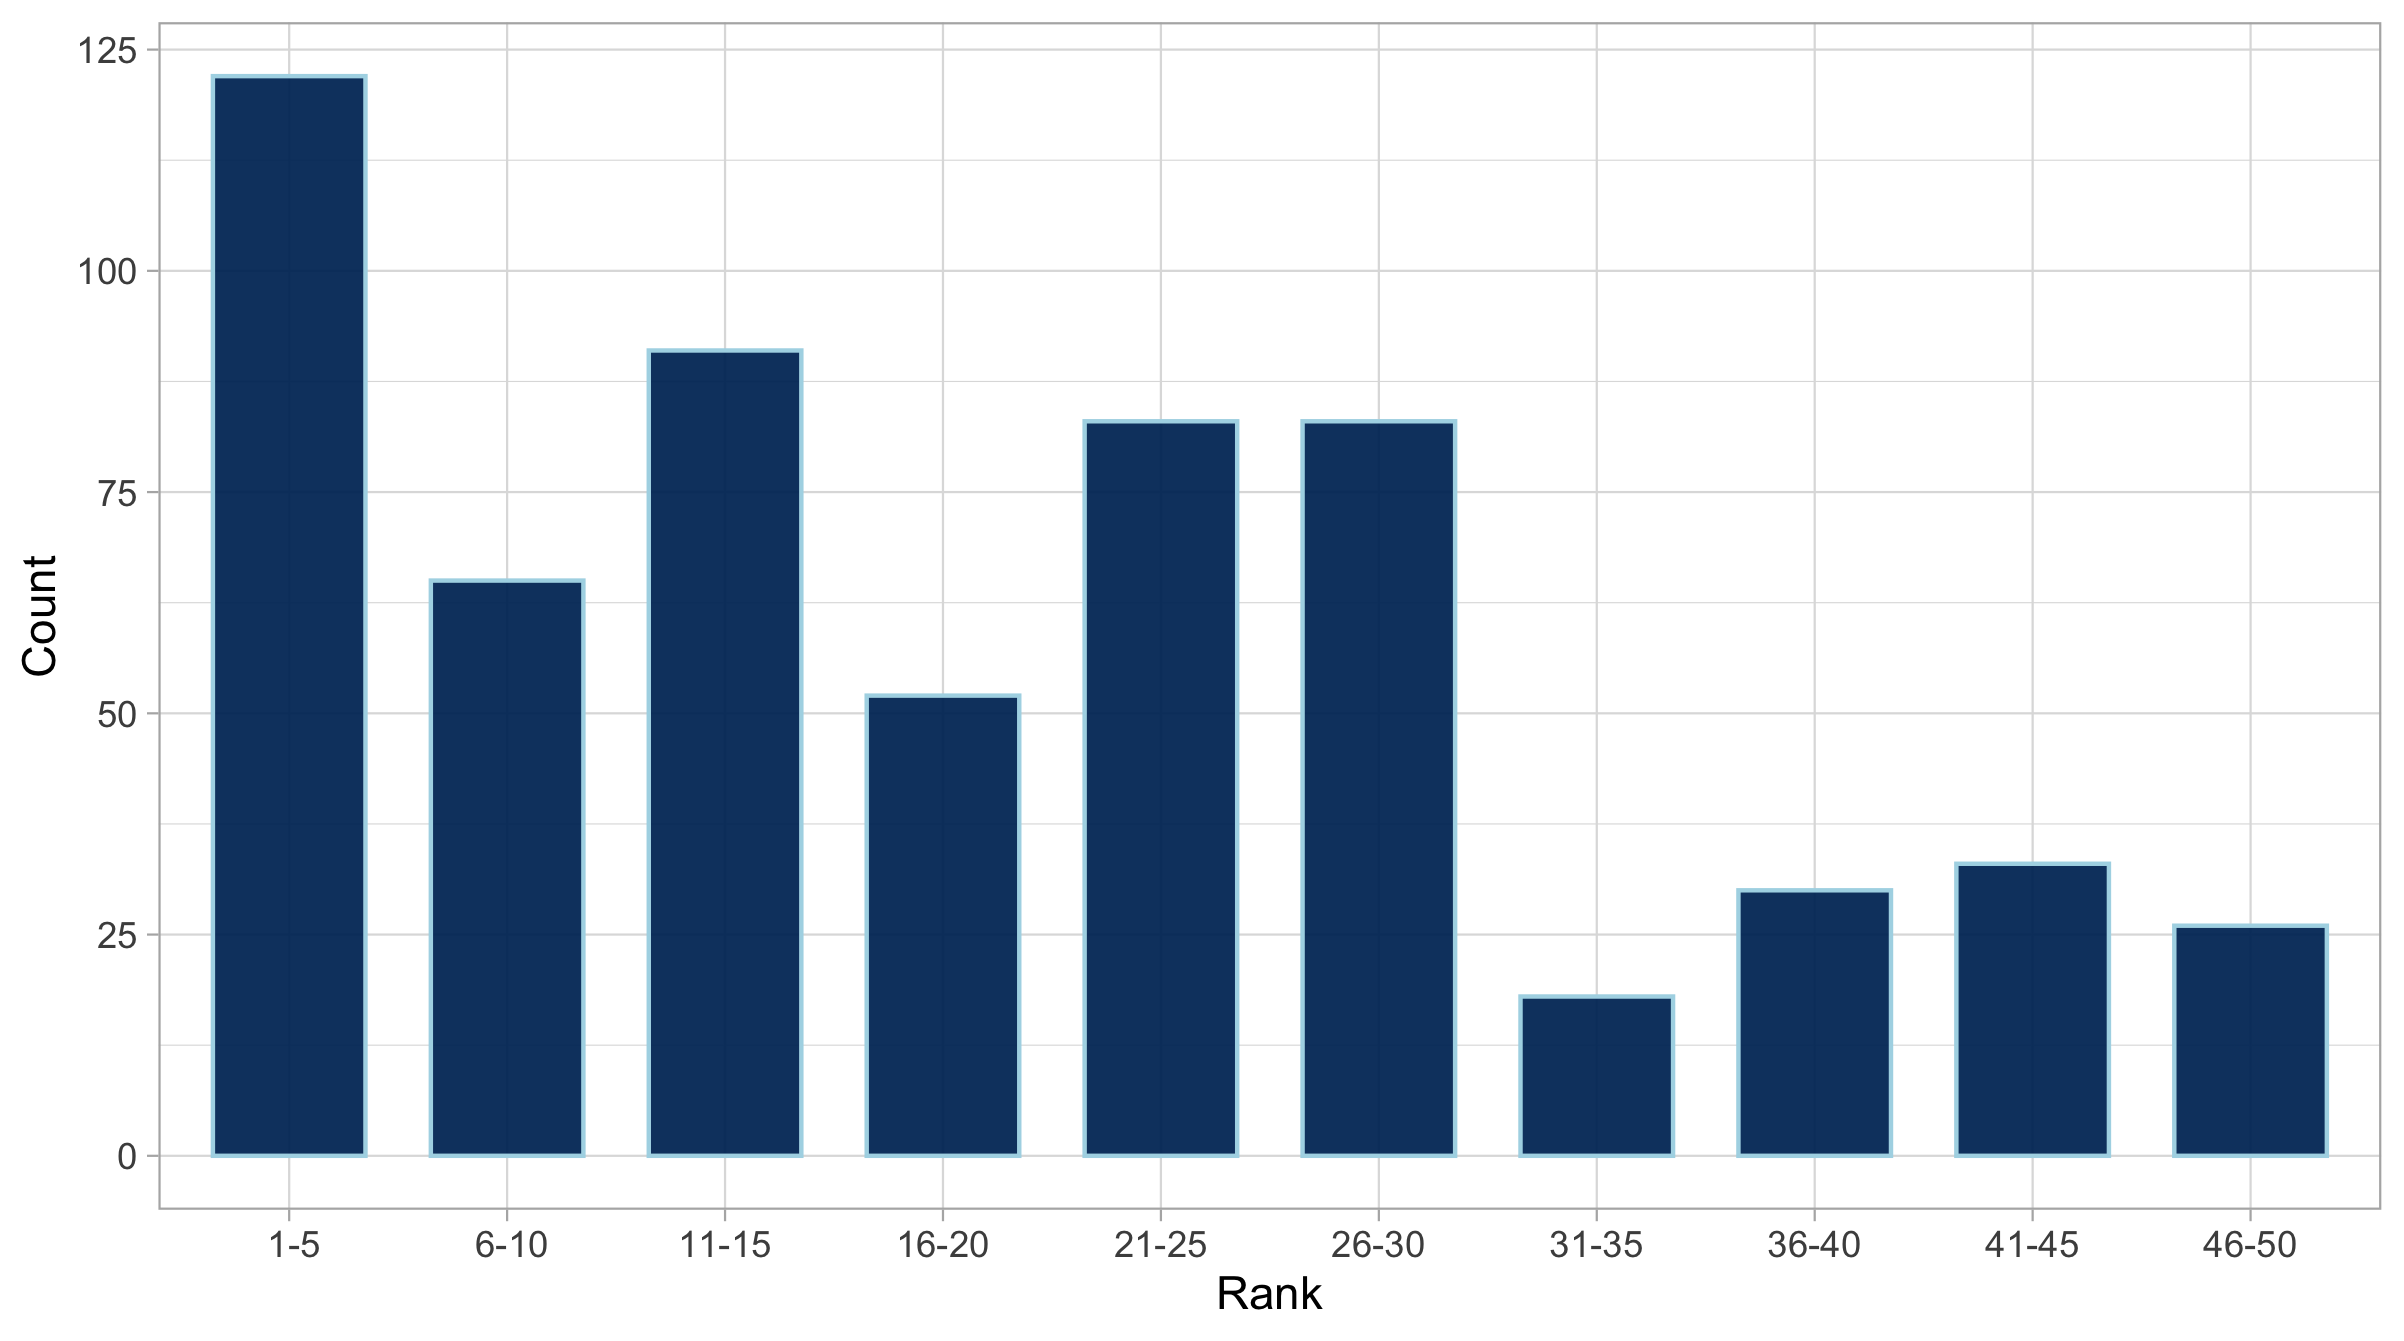
\includegraphics[width=140mm, scale=0.5]{fig/figure1.png}
    \end{center}
	\label{fig:figure1}
    \vspace{0.3cm}
    \begin{minipage}{0.95\textwidth} 
	{\footnotesize \textit{Note}: Figure presents the number of Ph.D. candidates by the program rankings. 50 Ph.D. programs are divided into 10 rank tiers. Note that there does not have to be 5 schools in each tier, for example, the tier 1 to 5 has 7 programs tied for first place.
	\par
	}
	\end{minipage}
\end{figure}

The number of Ph.D. candidates is evenly distributed across top 30 programs, ranging from 70 to 90, while the average number of Ph.D. graduates from schools from top 30 to 50 is relatively small, accounting for only 17.7 percent of the total. Our results are quite different from previous studies, with the top 5 programs accounting for about one-fifth of the job market in 2016-2017 by all 50 programs, and the top 15 for about half \citep{pathtoeconphd}. Factors associated with higher attrition in lower-ranked programs are lower attendance and lack of financial aid during graduate study, all of which are associated with other measures of student quality \citep{stock2014}. In this paper, we primarily divide students into two groups, students graduated from American undergraduate institutions (hereinafter referred to as American students, regardless of nationality), and International undergraduate institutions. International students’ origins are also categorized according to the region of their undergraduate institution. After obtaining the candidates’ public CV data from the department website, several pre-doctoral experiences are recorded for each CV (e.g. major, honors, international, and gender).

Our second source of data is the QS World University Rankings 2016, which is closest to where most of the candidates in our sample were when they enrolled. The rankings are used only to measure the quality of general undergraduate schools, and they are not applied to some of the specialized economics institutions (e.g. Bocconi, New Economics School, and Higher Economics School)  and liberal arts schools (e.g. Williams College) in the sample. When there is a range in the ranking, we take the midpoint of that range. While there has been debate about the reliability of ranking agencies and which rankings are better, QS rankings are the only ranking data available for 2016, based on a survey of more than 700 global universities.

\subsection{American vs International}
We measure the pre-doctoral experiences in several perspectives. We compare students from American undergraduate institutions and international students. Table 1 shows summary statistics of key variables of this perspective. The economics background variables, fields of study, are equal to one if the candidate has completed a bachelor's or master's degree in economics, business or public policy, and similarly, the math background variables are equal to 1 if the candidate holds a degree in mathematics, statistics or computer science. Of the 603 Ph.D. candidates for 2021-2022 job market, 374 of the candidates are international (62 percent). 427 (71 percent) of the candidates are male. Comparatively, 60 percent of American students have math background while only 19 percent of international do. Having a previous graduate degree differs noticeably, showing that most of the international students finish their master degree before a Ph.D. while only 18 percent of American students have a previous graduate degree. American candidates are more likely to have full-time RA experience than international candidates, with an average of 12 percent.
\begin{table}[h]\centering
\def\sym#1{\ifmmode^{#1}\else\(^{#1}\)\fi}
\caption{Descriptive Statistics: American vs International}
\resizebox{\columnwidth}{!}{
\begin{tabular}{l*{3}{c}}
\hline\hline
                    &\multicolumn{1}{c}{American}&\multicolumn{1}{c}{International}&\multicolumn{1}{c}{Combined}\\
                    &     Mean(SD)&     Mean(SD)&     Mean(SD)\\
\hline
\textit{Undergraduate fields of study} & & & \\
\quad Has a background in economics&        0.90&        0.95&        0.93\\
                    &      (0.31)&      (0.22)&      (0.26)\\
\quad Has a background in math&        0.60&        0.19&        0.35\\
                    &      (0.49)&      (0.39)&      (0.48)\\
\quad Has a background in economics and math&        0.55&        0.18&        0.32\\
                    &      (0.50)&      (0.38)&      (0.47)\\
\quad No background in math or economics&        0.06&        0.03&        0.04\\
                    &      (0.23)&      (0.18)&      (0.20)\\
\quad Has undergraduate honors&        0.45&        0.28&        0.34\\
                    &      (0.50)&      (0.45)&      (0.48)\\
\textit{Post-baccalaureate experience } &&&\\
\quad Has full time RA experiences&        0.28&        0.16&        0.21\\
                    &      (0.45)&      (0.37)&      (0.40)\\
\quad Has professional experiences&        0.15&        0.14&        0.14\\
                    &      (0.36)&      (0.35)&      (0.35)\\
\quad Has a previous graduate degree&        0.18&        0.79&        0.56\\
                    &      (0.38)&      (0.41)&      (0.50)\\
\textit{Rankings} &&&\\

\quad PhD program ranking (US) &       18.20&       18.96&       18.67\\
                    &     (14.28)&     (13.55)&     (13.83)\\
\quad Undergraduate institution ranking (World) &      163.58&      215.74&      196.01\\
                    &    (190.76)&    (189.59)&    (191.49)\\
\quad Attended an unranked undergraduate institution&        0.13&        0.21&        0.18\\
                    &      (0.33)&      (0.41)&      (0.38)\\
Female              &        0.26&        0.31&        0.29\\
                    &      (0.44)&      (0.46)&      (0.46)\\
\hline
Observations        &         229&         374&         603\\
\hline\hline
\end{tabular}}
\vspace*{0.09cm}
\begin{minipage}{0.95\textwidth} 
{\footnotesize 
\textit{Note}: Table presents the summary statistics. The first column surveys the candidates graduated from American undergraduate institutions, the second column focuses on the candidates graduated from foreign undergraduate institutions, and the third column shows the combined statistics. All variables except for the PhD program ranking and Undergraduate institution ranking are dummy variables. Standard errors are in parentheses.}
\end{minipage}
\end{table}

Interestingly, the diverse origins of the candidates did not significantly affect their program rankings, with both U.S. and international students averaging around 18th in the Ph.D. program rankings. As shown in Figure 2, the proportion of international candidates is evenly distributed among different rank tiers. However, International students' undergraduate institutions ranked 60 places lower than American students', given total 700 global universities were ranked in 2016. Compared to 21 percent for international students, 13 percent of American students come from unranked undergraduate schools. In general, international students rank lower than American students in undergraduate institutions, but their doctoral programs rank similar. 
\begin{figure}[H]
    \begin{center}
    \caption{Percentage of International Candidates by Program Rankings}
    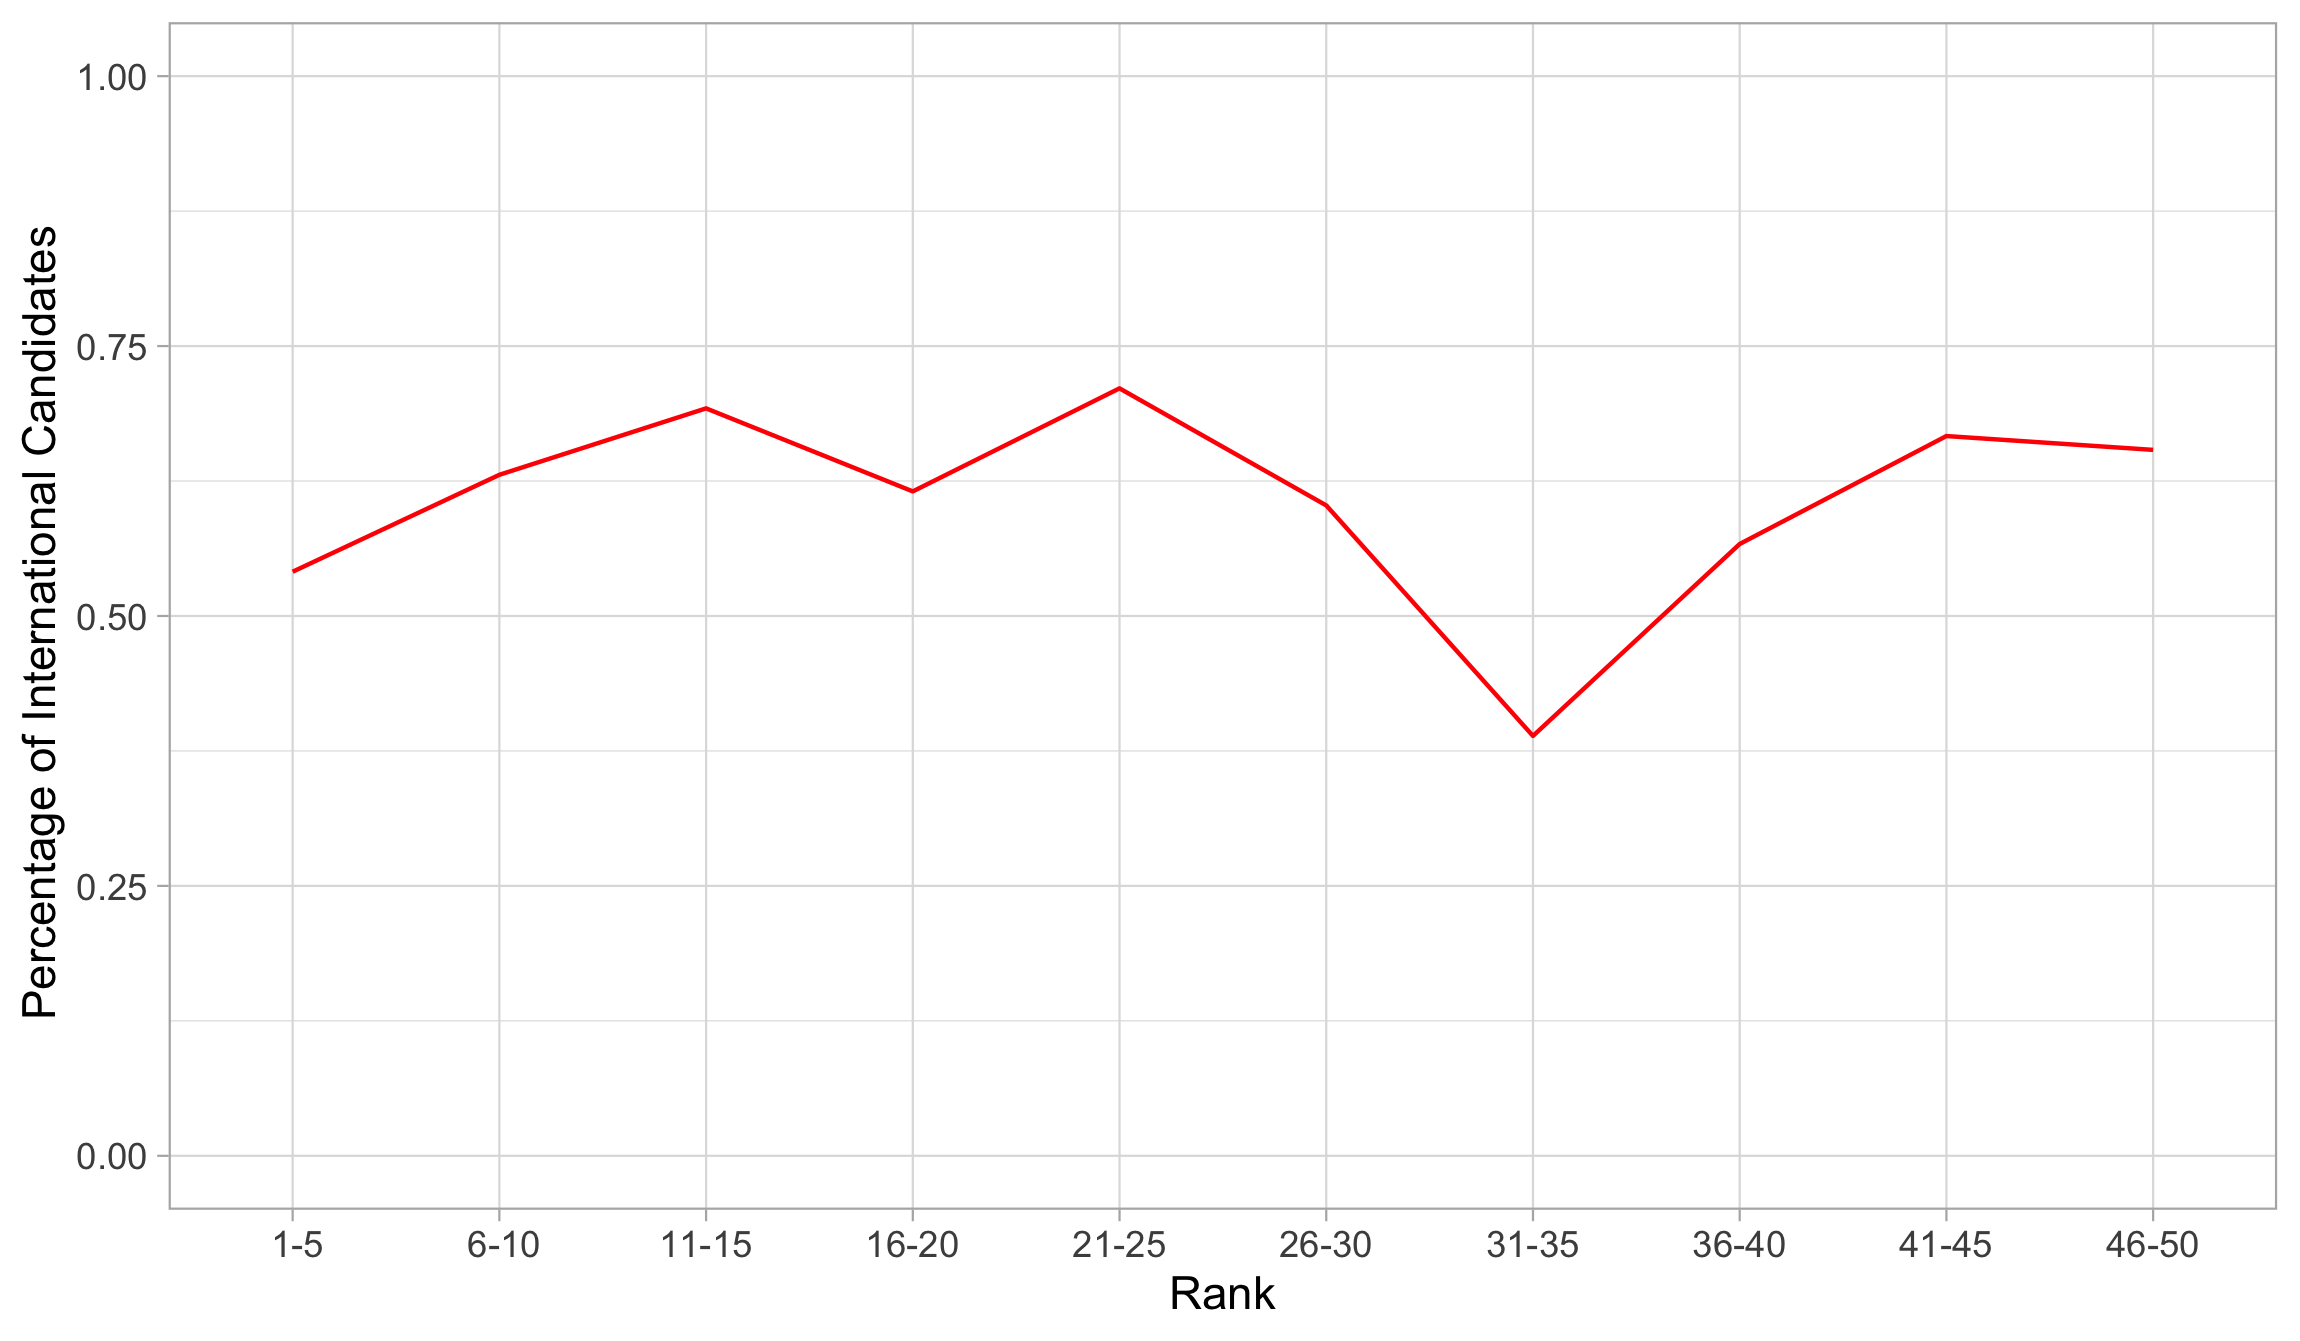
\includegraphics[width=100mm, scale=0.5]{fig/figure2.png}
    \end{center}
	\label{fig:figure1}
    \vspace{0.3cm}
    \begin{minipage}{0.95\textwidth} 
	{\footnotesize \textit{Note}: Figure presents the percentage of international candidates by Ph.D. program rankings. 50 Ph.D. programs are divided into 10 rank tiers. Note that there does not have to be 5 schools in each tier, for example, the tier 1 to 5 has 7 programs tied for first place.
	\par
	}
	\end{minipage}
\end{figure}


\clearpage
\subsection{Liberal Arts Colleges and Economics Schools}
Although we use the QS World Rankings to measure the quality of undergraduate institutions, it may not fully reflect the strength of economics study, especially for those economics higher education institutions. Liberal arts colleges in the United States are usually have a unique quality measure system. Thus we code them as indicator variables.
\begin{table}[htbp]\centering
\def\sym#1{\ifmmode^{#1}\else\(^{#1}\)\fi}
\caption{Different Types of Undergraduate Institutions}
\resizebox{\columnwidth}{!}{
\begin{tabular}{l*{4}{c}}
\hline\hline
                    &\multicolumn{1}{c}{Liberal Arts}&\multicolumn{1}{c}{Economics Schools}&\multicolumn{1}{c}{Unranked Schools}&\multicolumn{1}{c}{Ranked Schools}\\
                    &     Mean(SD)&     Mean(SD)&      Mean(SD)&      Mean(SD)\\
\hline
Has full time RA experiences&        0.39&        0.25&        0.14&        0.20\\
                    &      (0.49)&      (0.44)&      (0.35)&      (0.40)\\
Has professional experiences&        0.19&        0.04&        0.21&        0.13\\
                    &      (0.40)&      (0.19)&      (0.41)&      (0.34)\\
Has a previous graduate degree&        0.11&        0.75&        0.76&        0.53\\
                    &      (0.32)&      (0.44)&      (0.43)&      (0.50)\\
PhD program ranking &       17.42&       11.43&       26.01&       17.41\\
                    &     (12.55)&      (8.72)&     (13.55)&     (13.63)\\
Female              &        0.36&        0.36&        0.29&        0.28\\
                    &      (0.49)&      (0.49)&      (0.45)&      (0.45)\\
\hline
Observations        &          36&          28&         108&         431\\
\hline\hline
\end{tabular}
}
\vspace*{0.09cm}
\begin{minipage}{0.95\textwidth} 
{\footnotesize 
\textit{Note}: Table presents the summary statistics of different types of undergraduate institutions. Four columns represent four different types of schools. All variables except for the PhD program ranking are dummy variables. Standard errors are in parentheses.}
\end{minipage}
\end{table}


There are 36 candidates graduated from liberal arts colleges, accounting for about 6 percent (Table 2), compared with an average of 10 percent from 1966 to 2003 \citep{stock2007}, although the sample we are using comes from top 50 programs instead of the sample covering all candidates, the result suggests a relative decline in the productivity of candidates in the liberal arts colleges. 39 percent of candidates from liberal arts college have full-time research associate experience, the most of any school category, but have few chances of having a previous graduate degree. However, surprisingly, the Ph.D. programs of candidates from liberal arts colleges did not rank very high, and tied with the ranked schools, at around 17th place. By contrast, candidates from economics schools have the highest average Ph.D. program ranking, at 11th place, which is very impressive considering a total of 28 observations.

\subsection{Sources of U.S Economics Ph.D.s}
The top 10 worldwide undergraduate institution that generated the most U.S. economics Ph.D. candidates from 2021-2022 job market are presented in Table 3. Compared with the results from 1997 to 2002 (Siegfried and Stock, 2007, Table 2), Harvard University remains in second place. However, the importance of foreign universities has increased further, with American universities accounting for four of the top 10 sources of Ph.D.s between 1997 and 2002. Now only two remain. Among foreign universities, Korean universities (top 1 and top 6) were replaced by Chinese universities, and the total number of Chinese universities increased from two to four. The main source of American Ph.D.s has shifted from American universities to Chinese ones.

\begin{table}[H]

\caption{Top 10 Worldwide Sources of Top 50 U.S. Economics Ph.D.s}
\centering
\fontsize{8}{10}\selectfont
\resizebox{\columnwidth}{!}{
\begin{tabular}{l l c}
\hline
\hline
\multicolumn{1}{l}{Country} &\multicolumn{1}{l}{University Name}&\multicolumn{1}{l}{Number of Candidates}\\
\hline
China & Peking University & 21\\
USA & Harvard University& 11\\
Italy & Bocconi University & 10\\
Russia & Higher School of Economics & 10\\
Mexico & Instituto Tecnológico Autónomo de México & 9\\
China & Tsinghua University & 9\\
USA & University of Chicago & 9\\
India & University of Delhi & 9\\
China & Fudan University& 8\\
China & Renmin University of China & 8\\
\hline
\end{tabular}}
\vspace*{0.09cm}
\begin{minipage}{0.95\textwidth} 
{\footnotesize 
\textit{Note}: Table presents the country and name of top 10 worldwide sources of top 50 U.S. Ph.D. programs. }
\end{minipage}
\end{table}


In table 4, we narrow the list of PhD programs we consider down from the top 50 to the top 10, and now, only 4 foreign institutions remain. The list is still dominated by research universities that offer Ph.D. degrees, with 49 candidates from our top 10 worldwide sources, meaning there is little concentration of undergraduate sources in a total of 187 candidates in the top 10 Ph.D. programs.

\begin{table}[H]

\caption{Top 10 Worldwide Sources of Top 10 U.S. Economics Ph.D.s}
\centering
\fontsize{8}{10}\selectfont
\resizebox{\columnwidth}{!}{
\begin{tabular}{l l c}
\hline
\hline
\multicolumn{1}{l}{Country} &\multicolumn{1}{l}{University Name}&\multicolumn{1}{l}{Number of Candidates}\\
\hline
USA & Harvard University & 9\\
China & Peking University & 6\\
UK & University of Cambridge & 5\\
USA & University of Chicago & 5\\
Italy & Bocconi University & 4\\
USA & Brown University & 4\\
USA & Georgetown University & 4\\
Russia & New Economics School & 4\\
USA & Princeton University& 4\\
USA & Stanford University & 4\\
\hline
\end{tabular}}
\vspace*{0.09cm}
\begin{minipage}{0.95\textwidth} 
{\footnotesize 
\textit{Note}: Table presents the country and name of top 10 worldwide sources of top 10 U.S. Ph.D. programs. }
\end{minipage}
\end{table}



\subsection{Origin of International Candidates}
We divide the foreign sources of U.S. Ph.D. candidates into six major regions, namely, Western Europe, Eastern Europe (CIS), Latin America, South Asia, and East Asia. The differences between the six regions are shown in Table 5. Not surprisingly, East Asia is the largest foreign source of candidates, led by China, Korea and Japan. It was followed by Ph.D. candidates from Latin America (70) and Western Europe (68). The other three regions had the lowest numbers, all between 20 and 30.

Given the ranking of Ph.D. programs of regions, candidates from Eastern Europe tend to get the best programs, though it's worth noting that most of them graduated from economics schools. Ph.D. candidates from Western Europe have an average Ph.D. program ranking of 13. The most surprising of these are candidates from Latin American , whose average program ranking is 17.4, higher than the international average of 19 (Table 1), somewhat changes our impression towards their economics education.

Candidates from East Asia and Western Europe have the highest average undergraduate rankings. South Asia and Latin America have the highest and lowest percentage of female candidates, respectively. Around 90 percent of the candidates from Latin America, Middle East, South Asia, and Western Europe have a previous graduate degree before a Ph.D.
\begin{table}[H]

\caption{Characteristics of Different Regions.}
\centering
\fontsize{8}{10}\selectfont
\begin{tabular}[t]{l|r|r|r|r|r}
\hline
\textcolor{black}{\textbf{region}} & \textcolor{black}{\textbf{obeservations}} & \textcolor{black}{\textbf{Ph.D. Rankings}} & \textcolor{black}{\textbf{Undergrad Rankings}} & \textcolor{black}{\textbf{Female}} & \textcolor{black}{\textbf{Master Degree}}\\
\hline
region\_east\_asia & 141 & 21.33333 & 141.6129 & 0.3617021 & 0.6524823\\
\hline
region\_eastern\_eu & 22 & 12.63636 & 354.2000 & 0.3636364 & 0.7272727\\
\hline
region\_latin\_america & 70 & 17.40000 & 357.6957 & 0.2142857 & 0.8857143\\
\hline
region\_middle\_east & 24 & 26.04167 & 402.0000 & 0.2500000 & 0.8750000\\
\hline
region\_south\_asia & 33 & 26.57576 & 424.5000 & 0.3939394 & 0.9090909\\
\hline
region\_western\_eu & 68 & 13.01471 & 166.9184 & 0.2941176 & 0.8970588\\
\hline
\end{tabular}
\end{table}


As shown in Figure 3, the major proportion of foreign candidates at each tier of the program rankings, except for those at tier 1 to 5, are from East Asia. In particular, more than 60 percent of international candidates at programs ranked 30 to 40 are from China, South Korea, and Japan. Candidates from Western Europe tend to rank high overall.

\begin{figure}[H]
    \begin{center}
    \caption{Percentage of Candidates by Regions Along with the Program Ranking}
    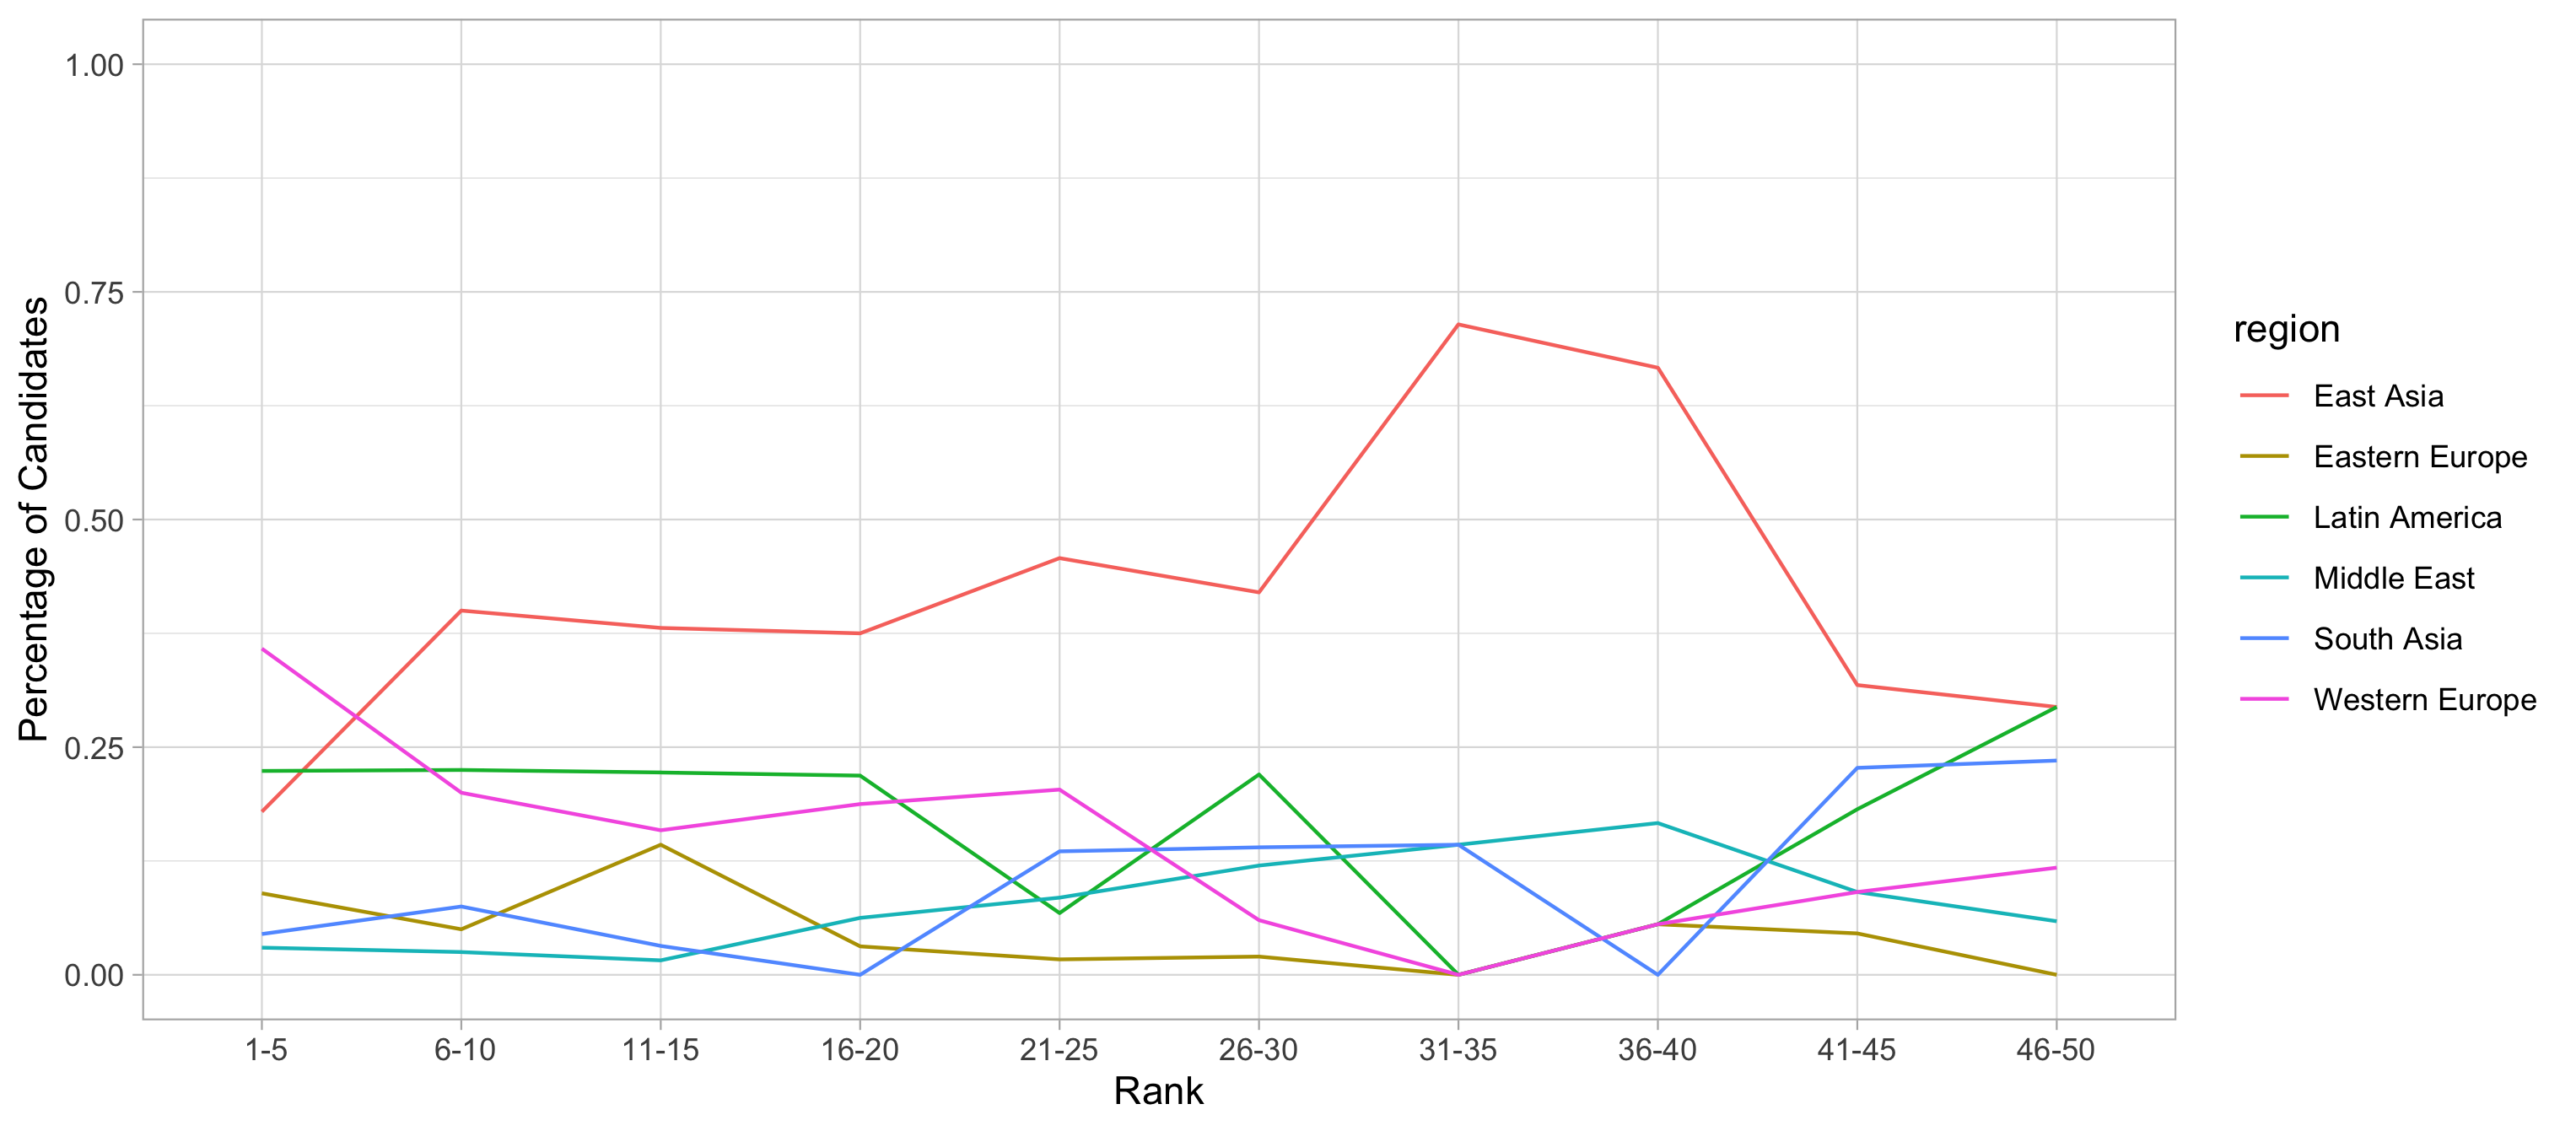
\includegraphics[width=140mm, scale=0.5]{fig/figure3.png}
    \end{center}
	\label{fig:figure1}
        \vspace{0.3cm}
    \begin{minipage}{0.95\textwidth} 
	{\footnotesize \textit{Note}: Figure presents the percentage of candidates from different regions by the program rankings. 50 Ph.D. programs are divided into 10 rank tiers. Note that there does not have to be 5 schools in each tier, for example, the tier 1 to 5 has 7 programs tied for first place.
	\par
	}
	\end{minipage}
\end{figure}




\clearpage
\section{Empirical Results \label{sec:empircal}}
Constrained by the volume and lack of complexity of the data, we choose to use simple multiple OLS linear regression to examine the impact of multiple characteristics on the ranking of PhD programs. The dependent variable is the Ph.D. program ranking, ranging from 1 to 50. The independent variables, except for the undergraduate institution ranking, that ranging from 1 to 700, are all indicator variables equal to 1 or 0. The independent variables are divided into four major panels, rankings and types of he undergraduate institution, undergraduate field of study, post-baccalaureate experience, and region of origin. 

Table 6 presents the results of our model. The first column ignores 172 observations that don’t have an undergraduate institution ranking. The second column did not control the rankings. The third column shows the complete results. We found that if an undergraduate institution moved up 100 places in the world rankings, the Ph.D. program of the candidate who graduated from that undergraduate institution would move up about 1.9 places in the national ranking. For instance, if a candidate graduated from an undergraduate institution ranked around 100 in the world, his or her doctoral program is likely to rank 1.9 places higher than that of a candidate with the same qualifications but graduated from an undergraduate school ranked at 200. The coefficient suggests that attending an unranked undergraduate school will lower candidates' Ph.D. program ranking by about 12 places, the effect is diminished if there is no control for the undergraduate institution ranking. 

Out of our expectation, attending an undergraduate liberal arts college or an undergraduate economics school has negative impacts on the Ph.D. program ranking, which is counter-intuitive to the descriptive analysis above. Graduating from an liberal arts college would possibly lower the Ph.D. program ranking by about 4.4 places although the result is only significant at 90 percent confidence level.

Having a background in economics is considered to have a negative impact on the Ph.D. program rankings, and having a math background improves the rankings. One possible explanation is that several candidates from top 1 to 10 programs \textit{incidentally} do not have a economics background. Actually, this issues may be very likely to happen, as the top 10 make up about 30 percent if the total candidates.

Having full time RA experiences before a Ph.D. was found to have positive effects on the Ph.D. program rankings. Worked as a RA would make candidates' program ranking 2.5 places higher. In contrast, having a previous graduate degree deals negative impacts, causing 2.3 places lower rankings. Having professional experiences has no effects. 

When it comes to the influence of regional origins on doctoral program rankings, some regions, such as Western Europe, Eastern Europe, and Latin America, have a huge advantage over others. Candidates from Eastern Europe ranked on average 8.23 places higher than those from regions not listed (North America and Australia). South Asia, East Asia and the Middle East had no effect on the ranking. The estimate for the effect of Female is negative and insignificant for the rankings.



\begin{table}[htbp]\centering
\def\sym#1{\ifmmode^{#1}\else\(^{#1}\)\fi}
\caption{PhD program rankings with pre-doctoral characteristics}
\resizebox{\columnwidth}{!}{
\begin{tabular}{l*{3}{c}}
\hline\hline
                    &\multicolumn{1}{c}{PhD program ranking}&\multicolumn{1}{c}{PhD program ranking}&\multicolumn{1}{c}{PhD program ranking}\\
\hline
\textit{Rankings and types of undergraduate institution} & & & \\

\quad Undergraduate institution ranking&       0.019\sym{***}&                     &       0.019\sym{***}\\
                    &     (0.004)         &                     &     (0.003)         \\
[1em]
\quad Attended an unranked undergraduate institution&                &       7.247\sym{***}&      11.945\sym{***}\\
                    &                  &     (1.516)         &     (1.688)         \\
[1em]
\quad Attended an undergraduate liberal arts college&              &       1.246         &       4.438\sym{*}  \\
                    &                &     (2.257)         &     (2.313)         \\
[1em]
\quad Attended an undergraduate economics school&             &      -1.567         &       2.885         \\
                    &                  &     (3.057)         &     (3.085)         \\
\textit{Undergraduate fields of study} & & & \\
[1em]
\quad Has a background in economics&       6.032\sym{***}&       5.503\sym{***}&       4.864\sym{***}\\
                    &     (1.879)         &     (1.882)         &     (1.749)         \\
[1em]
\quad Has a background in math&      -1.541         &      -1.385         &      -1.719         \\
                    &     (1.430)         &     (1.307)         &     (1.273)         \\
\textit{Post-baccalaureate experience} & & & \\
[1em]
\quad Has full time RA experiences&      -2.622         &      -3.195\sym{**} &      -2.578\sym{*}  \\
                    &     (1.646)         &     (1.402)         &     (1.383)         \\
[1em]
\quad Has professional experiences&       1.710         &      -0.059         &       0.150         \\
                    &     (2.147)         &     (1.725)         &     (1.710)         \\
[1em]
\quad Has a previous graduate degree&       3.224\sym{**} &       2.498\sym{*}  &       2.334\sym{*}  \\
                    &     (1.440)         &     (1.304)         &     (1.257)         \\
\textit{Region of Origin} & & & \\
[1em]
\quad Western Europe      &      -8.194\sym{***}&      -7.310\sym{***}&      -7.586\sym{***}\\
                    &     (2.332)         &     (2.097)         &     (2.066)         \\
[1em]
\quad Eastern Europe      &      -8.646         &      -6.530\sym{*}  &      -8.234\sym{**} \\
                    &     (8.224)         &     (3.934)         &     (3.939)         \\
[1em]
\quad South Asia          &      -1.451         &       4.082         &       0.430         \\
                    &     (3.394)         &     (2.737)         &     (2.768)         \\
[1em]
\quad East Asia           &       2.178         &       1.575         &       1.927         \\
                    &     (1.629)         &     (1.563)         &     (1.510)         \\
[1em]
\quad Latin America       &      -7.500\sym{***}&      -4.474\sym{**} &      -7.336\sym{***}\\
                    &     (2.611)         &     (2.172)         &     (2.211)         \\
[1em]
\quad Middle East         &      -0.485         &       2.691         &       0.024         \\
                    &     (3.926)         &     (2.812)         &     (2.757)         \\
[1em]
Female              &       0.988         &       0.717         &       1.349         \\
                    &     (1.399)         &     (1.182)         &     (1.148)         \\
[1em]
Constant            &       8.277\sym{***}&      12.691\sym{***}&       9.853\sym{***}\\
                    &     (2.304)         &     (2.147)         &     (2.050)         \\
\hline
Observations        &         431         &         603         &         603         \\
\(R^{2}\)           &       0.152         &       0.141         &       0.183         \\
\hline\hline
\end{tabular}}
\vspace*{0.09cm}
\begin{minipage}{0.95\textwidth} 
{\footnotesize 
The table presents the results. Reported coefficients are marginal effects for OLS multi-linear regression models. The first column ignores 172 observations that don't have an undergraduate institution ranking. The second column did not control the rankings. The third column shows the complete results. All variables except for undergraduate institution ranking are dummy variables. Standard errors are in parentheses. \sym{*} \(p<0.1\), \sym{**} \(p<0.05\), \sym{***} \(p<0.01\)}
\end{minipage}

\end{table}


\clearpage
\section{Conclusion \label{sec: conclusion}
}
This paper primarily analyze how would the origin and types of the undergraduate institutions affect candidates' Ph.D. program rankings. The proportion of international Ph.D. candidates has been increasing in recent years, and the growing importance of international candidates requires researchers to pay more attention to the differences between them and American candidates. 

Using the CV data, we find that unlike American candidates, international candidates are more likely to have a previous graduate degree before a Ph.D., and less likely to have full time RA experiences and a background in math. Candidates who come from a highly ranked undergraduate institution, have full time RA experiences, and come from Western Europe, Eastern Europe, or Latin America, are more likely to graduate from highly ranked Ph.D. programs, while attending an unranked undergraduate institution and an liberal arts college have negative effects on Ph.D. program rankings.

One of the more salient conclusions of this study is that, worldwide, China become the leading incubator of future top 50 U.S. economics Ph.D.s. When narrowing the list to top 10, Harvard University tops the list of undergraduate
institutions attended by eventual Ph.D.s in economics, and U.S. universities are the major sources. The relatively small number of candidates from top sources also implies the little concentration of undergraduate schools attended by top 10 program candidates.

%%%%%%%%%%%%%%%%%%%%%%%%%%%%%%%%%%%%%%%%%%%%%%%%%
\clearpage
\begin{singlespace}
%\bibliographystyle{plainnat}
%\bibliographystyle{chicago}
\bibliographystyle{aer}
\bibliography{our-cites.bib}
\end{singlespace}
%%%%%%%%%%%%%%%%%%%%%%%%%%%%%%%%%%%%%%%%%%%%%%%%%


%%%%%%%%%%%%%%%%%%%%%%%%%%%%%%%%%%%%%%%%%%%%%%%%%
%%%%% These commands start the appendix and change the Table & Figure numbering
\newpage
\appendix
\setcounter{table}{0}
\renewcommand{\tablename}{Appendix Table}
\renewcommand{\figurename}{Appendix Figure}
\renewcommand{\thetable}{A\arabic{table}}
\setcounter{figure}{0}
\renewcommand{\thefigure}{A\arabic{figure}}
%%%%%%%%%%%%%%%%%%%%%%%%%%%%%%%%%%%%%%%%%%%%%%%%%




\end{document}
